\documentclass[conference]{IEEEtran}
\IEEEoverridecommandlockouts
\usepackage{cite}
\usepackage{amsmath,amssymb,amsfonts}
\usepackage{algorithmic}
\usepackage{graphicx}
\usepackage{textcomp}
\usepackage{xcolor}
\usepackage{balance}
\def\BibTeX{{\rm B\kern-.05em{\sc i\kern-.025em b}\kern-.08em
    T\kern-.1667em\lower.7ex\hbox{E}\kern-.125emX}}
\begin{document}

\title{Causal Diagnosis of Reinforcement Learning Performance in Vision-Based Multi-Robot Task Allocation with a Digital Twin}

\author{\IEEEauthorblockN{1\textsuperscript{st} Yan Santos Leite}
\IEEEauthorblockA{\textit{School of Electrical, Mechanical and Computer Engineering} \\
\textit{Universidade Federal de Goiás (UFG)}\\
Goiânia, Brazil \\
santosleiteyan@gmail.com}
\and
\IEEEauthorblockN{2\textsuperscript{nd} Alisson Assis Cardoso}
\IEEEauthorblockA{\textit{School of Electrical, Mechanical and Computer Engineering} \\
\textit{Universidade Federal de Goiás (UFG)}\\
Goiânia, Brazil \\
alsnac@ufg.br}
}

\maketitle

\begin{abstract}
Multi-robot task allocation (MRTA) is commonly solved with greedy heuristics that are fast but cannot anticipate future demand. We train a reinforcement learning (RL) agent (Proximal Policy Optimization, PPO) for this task, with observations grounded in a camera-based digital twin: an overhead camera and a YOLOv8n detector localize a fleet of TurtleBot3 robots with a mean tracking error of 4.7 cm (mAP@0.5 = 0.995), replacing raw odometry as the position source for the allocation policy. We compare PPO against the greedy \textit{nearest-free} heuristic using rigorous paired statistical tests over 1000 episodes. Contrary to our hypothesis, PPO did not outperform nearest-free: mean response time was about 12\% worse, a statistically significant difference. We found that PPO assigns tasks to busy robots in 4.0\% of decisions, versus 0.3\% for nearest-free (13 times higher), suggesting the training penalty was insufficient to teach this constraint. We tested this causally with \textit{action masking}, which structurally prevents the policy from choosing busy robots: the invalid-assignment rate dropped to exactly 0\%, but response time remained about 11\% worse than nearest-free. The constraint violation is therefore not the dominant cause of the gap. We report this negative result and its root-cause diagnosis with full statistical rigor, arguing that a falsified hypothesis, tested transparently, is more valuable than an incomplete positive claim.
\end{abstract}

\begin{IEEEkeywords}
multi-robot task allocation, multi-robot systems, deep reinforcement learning, proximal policy optimization, action masking, digital twin, object detection, negative result
\end{IEEEkeywords}

\section{Introduction}

Coordinating a fleet of mobile robots to service spatially and temporally distributed demands (multi-robot task allocation, MRTA) is a core problem in multi-robot coordination~\cite{gerkey2004formal}, with applications spanning service robotics to warehouse automation~\cite{agrawal2022dcmrta,pal2025together}. Greedy heuristics such as nearest-free assignment are simple, fast, and respect operational constraints (e.g., never assigning a busy robot) by construction. Their problem is that they only look at the current demand: they assign the closest idle robot without considering that this same robot might be better used, more efficiently, for a demand that arrives shortly after. Reinforcement learning (RL) is a natural candidate to correct this myopia, since a learned policy can, in principle, trade a locally suboptimal assignment for a globally better outcome.

There is a second, largely independent challenge. To decide which robot to send, the allocator needs to know where each robot currently is, and obtaining that in real time is neither trivial nor free. Wheel odometry, the simplest method, estimates position from how much the wheels have turned, and accumulates error over time. More precise methods, such as SLAM, correct for that drift but are expensive to deploy on real hardware. We use a low-cost alternative: a ceiling-mounted camera observing the operating area, with a YOLOv8n detector that identifies each robot in the image. We call this system a \emph{digital twin}: it publishes each robot's position in real time, without accumulating error over time.

This paper makes two contributions. First, we integrate and validate this camera-based digital twin (4.7 cm mean localization error, mAP@0.5 = 0.995) to feed the observations of an RL-based allocator, validating the full pipeline on three TurtleBot3 Waffle robots in Gazebo. Second, and most importantly, we report a \emph{negative result}: our PPO-trained agent does not outperform the nearest-free heuristic. Investigating why, we found a concrete lead: PPO assigns tasks to busy robots 13 times more often than the heuristic, which seemed to explain the problem. We tested this explanation directly with \textit{action masking}: instead of only penalizing this choice in the reward and hoping PPO would learn to avoid it on its own, we removed busy robots from the set of valid options at every decision, making that choice impossible by construction (the same principle that already makes nearest-free immune to this error). We found that this structural fix was not the main cause --- performance barely improved. This full process --- a plausible hypothesis, tested and then refuted with data --- is the paper's main contribution: showing transparently not just that the method failed, but why it failed.

\section{Related Work}

Classical MRTA relies on market-based auctions~\cite{dias2006market}, greedy assignment~\cite{gerkey2004formal}, and centralized optimization, which offer strong constraint guarantees but limited foresight. Learning-based allocation has also been explored in multi-agent CTDE formulations~\cite{lowe2017multi}, in addition to single-agent settings such as ours. Reproducibility and evaluation rigor remain open problems in deep RL~\cite{henderson2018deep}: variance across random seeds alone can produce statistically significant differences, motivating significance testing rather than comparing average returns alone, a gap we address with paired tests. Orr and Dutta~\cite{orr2023survey} survey multi-agent RL applications in multi-robot systems, identifying scalability and the lack of standardized simulation benchmarks as open challenges. Recent RL-based warehouse MRTA includes decentralized MDP approaches~\cite{agrawal2022dcmrta} and dual-agent frameworks~\cite{pal2025together}; unlike these, our focus is diagnosing \emph{why} a learned policy fails to beat a greedy heuristic, via a causal experiment (action masking). On perception, YOLO-family detectors~\cite{yolov8} are common for vision-based tracking~\cite{ahmed2021topview}, but prior work evaluates detection quality in isolation, without ablating its effect on a learned allocation policy while holding all else fixed --- the ablation we run here. Negative-result reporting remains rare in robotics and RL; we follow Henderson et al.'s calls for rigorous paired statistical evaluation~\cite{henderson2018deep}. Our causal diagnosis also draws on Huang and Ontañón~\cite{huang2022masking}, who show that action masking produces a valid policy gradient and outperforms soft penalization of invalid actions. Unlike that RTS setting, where masking closes the performance gap, in our domain it eliminates the structural violation without closing the gap --- evidence that the underlying cause differs.

\section{Digital Twin and RL Formulation}

The digital twin consists of a statically mounted overhead camera, a YOLOv8n detector fine-tuned on 375 manually annotated frames (one to three TurtleBot3 Waffle robots), and a coordinate-projection module mapping bounding-box centers to world-frame $(x,y)$ positions, published on ROS2 topic \texttt{/robot\_detections}. The detector reaches mAP@0.5 = 0.995 with 36 ms/frame inference on CPU. A static 8-pose benchmark gives 1.24 cm mean error; over a continuous multi-robot tracking sequence (2031 samples, live Nav2 navigation) the mean error is 4.7 cm, with 100\% of detections within 15 cm of ground truth (Fig.~\ref{fig:digitaltwin}) --- the roughly $4\times$ increase from static to dynamic is consistent with motion blur and detection-to-pose latency, not a detector limitation. This dynamic error is the precision level used in all downstream experiments.

\begin{figure}[htbp]
\centerline{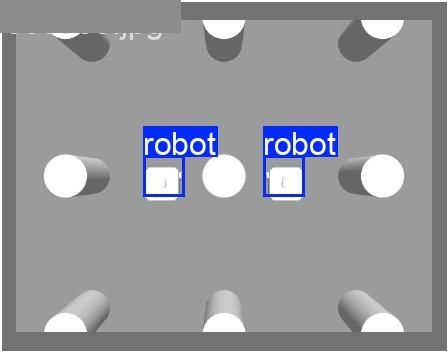
\includegraphics[width=0.85\linewidth]{fig_yolo_labels_crop.jpg}}
\centerline{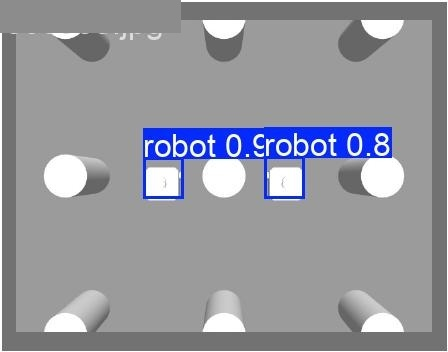
\includegraphics[width=0.85\linewidth]{fig_yolo_pred_crop.jpg}}
\caption{Two of the fleet's TurtleBot3 Waffle robots as seen by the overhead camera: ground-truth annotation (top) vs.\ detector prediction (bottom) in a scene from the validation set. Full three-robot experiments are quantified in Sections~IV--V.}
\label{fig:robots}
\end{figure}

\begin{figure}[htbp]
\centerline{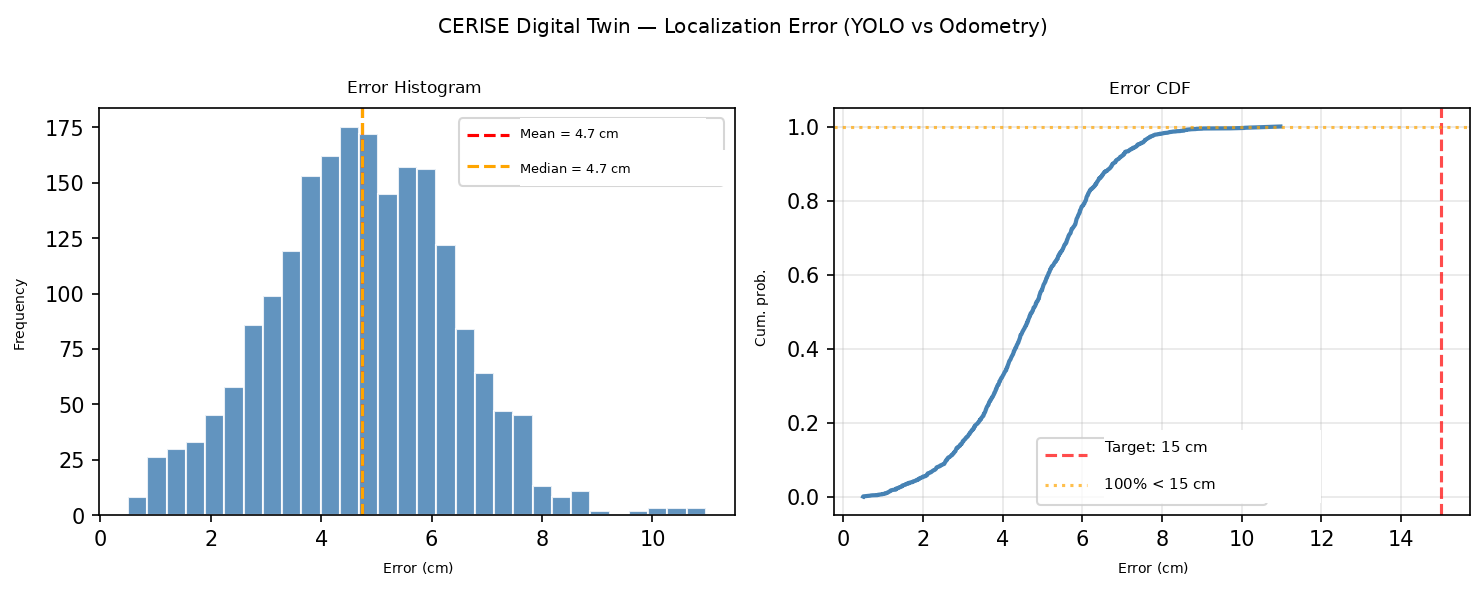
\includegraphics[width=\linewidth]{fig_digitaltwin.png}}
\caption{Digital twin localization error over a continuous multi-robot tracking sequence. Mean error is 4.7 cm; 100\% of detections fall within 15 cm of ground truth.}
\label{fig:digitaltwin}
\end{figure}

We formulate task allocation as a Markov Decision Process (MDP): at each new demand arrival, a single centralized agent decides, based on the current state of the system, which of $N=3$ robots services it. The 21-dimensional state describes everything the agent observes at that instant: each robot's $(x,y)$ position (from the digital twin or odometry, depending on the experimental arm), how long until each robot becomes free, the origin and destination of the demand that just arrived, and the origin and destination of the next two demands already visible in the queue, a lookahead signal that lets the agent weigh the future impact of each choice, not just the immediate demand. The action is the discrete choice of which of these $N$ robots should service the current demand. The reward is the negative response time $r = -(t_{\text{wait}} + t_{\text{travel}})$: the faster a demand is serviced, from arrival until the chosen robot starts executing it, the higher the reward. This corrects an earlier formulation that penalized only travel time to the demand, ignoring how long the chosen robot would still take to become free; under that formulation, a busy-but-nearby robot could look as good as an idle-but-distant one, which under-weights queueing and biases the policy toward idle robots even when they are far away. We train with PPO~\cite{schulman2017proximal} via Stable-Baselines3~\cite{stable-baselines3} for 500{,}000 timesteps ($\sim$2h on CPU), at library default hyperparameters (Table~\ref{tab:hparams}) to isolate the effect of observation source and masking rather than PPO tuning; Gazebo is reserved for final-stage physical validation, not training. Both PPO variants learn (Fig.~\ref{fig:learning}): mean episodic reward improves from $\sim{-21}$ to $\sim{-17.7}$ over 500k steps, but neither crosses the nearest-free reference ($-16.7$); PPO(odom) converges slightly faster, confirming the 4.7 cm digital-twin noise is a second-order effect.

\begin{table}[htbp]
\caption{Training hyperparameters (identical across all variants)}
\begin{center}
\begin{tabular}{|l|c|}
\hline
\textbf{Hyperparameter} & \textbf{Value} \\
\hline
Policy / network & MlpPolicy, $\pi$=[64,64], $V$=[64,64] \\
\hline
Learning rate & $3\times10^{-4}$ \\
\hline
$n_{\text{steps}}$ (per env) / batch & 2048 / 64 \\
\hline
$\gamma$ / GAE $\lambda$ / clip range & 0.99 / 0.95 / 0.2 \\
\hline
Parallel envs / seed & 8 / 42 \\
\hline
\end{tabular}
\label{tab:hparams}
\end{center}
\end{table}

\begin{figure}[htbp]
\centerline{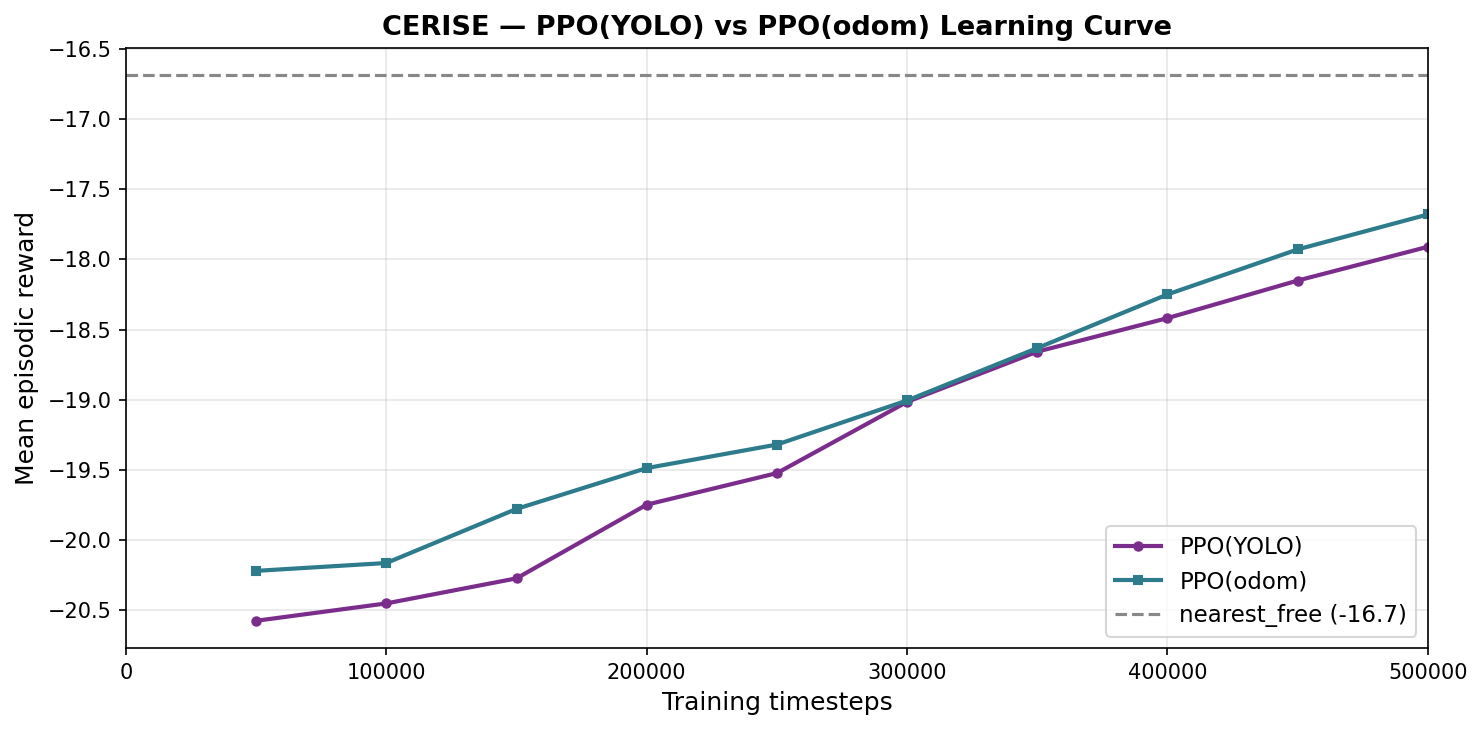
\includegraphics[width=\linewidth]{fig_learning.png}}
\caption{PPO learning curves for the YOLO and odometry observation variants, with the nearest-free baseline as a reference line.}
\label{fig:learning}
\end{figure}

\section{Experimental Setup}

We compare PPO against three baselines: \emph{random} and \emph{round-robin}, which serve as a performance floor with no notion of proximity or queueing, and \emph{nearest-free}, which assigns the closest idle robot and is infeasible by construction when none is idle. To isolate the digital-twin effect, we train PPO(YOLO) and PPO(odom), identical except for the position source used in the observation (4.7 cm Gaussian noise for YOLO vs.\ accumulated odometry drift for odom); using matched seeds across both variants ensures the only difference between them is that noise source, not training luck. Each comparison evaluates 1000 paired episodes, using the same demand sequence and seed for both policies, which lets us report not only whether the difference is statistically significant (Wilcoxon signed-rank) but also its effect size (Cliff's delta) and uncertainty (bootstrap confidence intervals). To check whether these conclusions hold under different demand pressures, a load sweep covers six inter-arrival regimes from 30s to 10s (500 episodes/point). The full pipeline, from camera to YOLO, through the allocator and Nav2, to the TurtleBot3 Waffle robots, was validated end-to-end on three robots in Gazebo Classic (ROS2 Humble); the RL policy itself, however, trains only in the analytical environment. To causally test whether the soft constraint of never assigning a busy robot drives PPO's poor performance, we additionally train PPO(YOLO, masked): identical to PPO(YOLO) except the action distribution is restricted every step to currently idle robots, via \textit{action masking}~\cite{huang2022masking} using sb3-contrib's MaskablePPO, with the same hyperparameters and training budget. We omit a PPO(odom, masked) variant since the digital-twin noise effect already proved second-order (Section~V), so testing it would not change the experiment's qualitative conclusion.

\section{Results}

Table~\ref{tab:ablation} summarizes moderate-load performance: nearest-free outperforms both PPO variants on all four reported metrics (mean latency, p95, makespan, and load imbalance), and the gap between PPO(YOLO) and PPO(odom) is small compared to how far either falls behind nearest-free, confirming the digital-twin noise is a second-order effect. The Wilcoxon test confirms this advantage is statistically significant in both comparisons ($p<0.001$, large Cliff's $\delta$). In a complementary analysis focused specifically on decisions where PPO and nearest-free choose different robots, nearest-free picks the better option in 72\% of those cases (2000 episodes). The p95-to-mean latency ratio is also similar across the three policies ($\approx$1.56--1.59, Fig.~\ref{fig:boxplot}), indicating that PPO's worse performance comes from a shift of the entire response-time distribution, not a tail of a few catastrophic episodes dragging the average down.

\begin{table}[htbp]
\caption{Policy comparison at moderate load (inter-arrival 12s, 1000 paired episodes)}
\begin{center}
\begin{tabular}{|l|c|c|c|c|}
\hline
\textbf{Policy} & \textbf{Mean lat.} & \textbf{p95 lat.} & \textbf{Makespan} & \textbf{Imbal.} \\
\hline
Nearest-free & \textbf{16.83 s} & \textbf{26.73 s} & \textbf{336.58 s} & \textbf{0.24} \\
\hline
PPO (YOLO) & 17.83 s & 27.84 s & 356.63 s & 0.32 \\
\hline
PPO (odom) & 17.12 s & 27.18 s & 342.34 s & 0.31 \\
\hline
\end{tabular}
\label{tab:ablation}
\end{center}
\end{table}

\begin{figure}[htbp]
\centerline{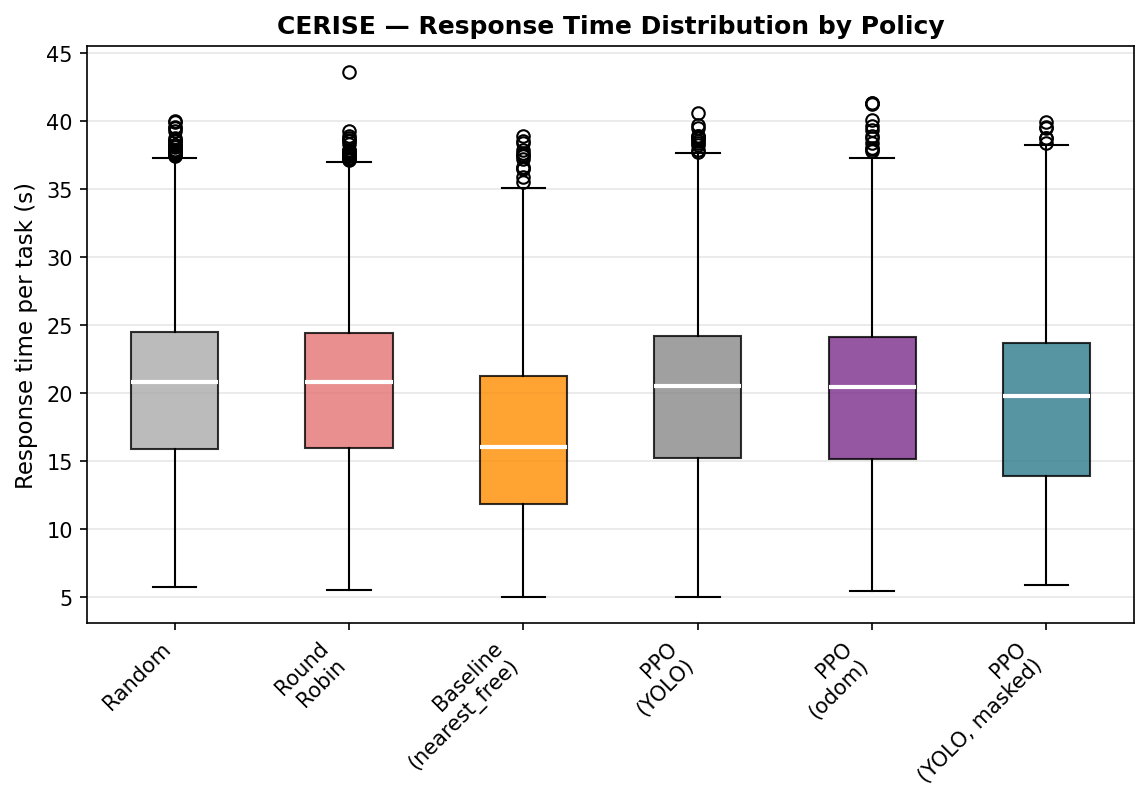
\includegraphics[width=\linewidth]{fig_boxplot.png}}
\caption{Response-time distribution across evaluated policies, including the masked PPO variant.}
\label{fig:boxplot}
\end{figure}

Table~\ref{tab:load} and Fig.~\ref{fig:load} show that PPO's disadvantage relative to nearest-free narrows as load increases, from +19.0\% at low load to +7.7\% at high load, though nearest-free remains faster throughout the tested range.

\begin{figure}[htbp]
\centerline{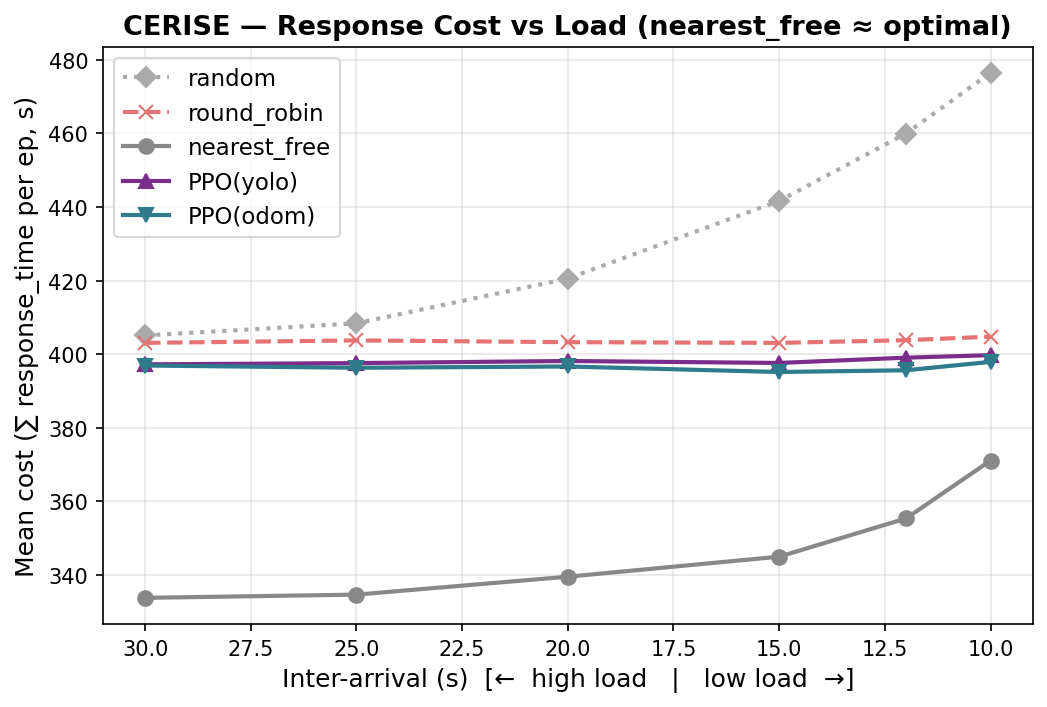
\includegraphics[width=\linewidth]{fig_load.png}}
\caption{Response time as a function of demand load (inter-arrival time) for nearest-free and PPO(YOLO).}
\label{fig:load}
\end{figure}

\begin{table}[htbp]
\caption{Response time by policy across load regimes}
\begin{center}
\begin{tabular}{|l|c|c|c|}
\hline
\textbf{Inter-arrival} & \textbf{Nearest-free} & \textbf{PPO(YOLO)} & \textbf{Difference} \\
\hline
30 s (low) & 333.8 s & 397.3 s & +19.0\% \\
\hline
12 s (mod.) & 355.4 s & 399.1 s & +12.3\% \\
\hline
10 s (high) & 371.1 s & 399.8 s & +7.7\% \\
\hline
\end{tabular}
\label{tab:load}
\end{center}
\end{table}

\section{Diagnosing the Negative Result}

PPO learns, and even gets a two-step demand lookahead the greedy baseline lacks, yet still fails to beat nearest-free. We investigated three explanations. Soft vs.\ hard constraint enforcement: nearest-free never assigns a busy robot, since that constraint is built into the algorithm itself; PPO can only learn to avoid this indirectly through the reward penalty, and still gets it wrong in 4.0\% of decisions versus 0.3\% for nearest-free, the largest single contributor we found. Limited action space: with only $N=3$ robots, few assignment combinations are meaningfully different, capping any anticipatory advantage; our advisor corroborated this as a plausible, if secondary, factor. Training budget: 500k steps produced clear learning but not convergence, though PPO's own response time stays nearly flat across load regimes (397--400 s, Table~\ref{tab:load}) while nearest-free's grows substantially under high load, suggesting the plateau is not purely a budget artifact.

Causal test. To test directly whether that constraint violation was the cause, we trained PPO(YOLO, masked) and re-evaluated it with unmasked PPO(YOLO) and nearest-free over a fresh 1000-episode run at moderate load, so all three policies were compared under identical conditions. Masking achieves its structural goal: the invalid-assignment rate drops from 4.0\% to exactly 0.0\%. Yet mean response time barely improves, from about 12\% worse than nearest-free without masking to about 11\% worse with it, roughly a 1-point gain. Nearest-free still significantly outperforms the masked variant ($p<0.001$, Cliff's $\delta=0.636$), an effect size of the same order of magnitude as without masking ($\delta=0.703$).

The causal hypothesis is refuted. The explanation that looked most plausible before the test does not hold up: eliminating the violation by construction barely closes the gap. Weight shifts back to the small action space and training budget, and a further hypothesis emerges: by preventing the policy from even considering busy robots, masking also removes any learning signal about the consequence of that choice, which may reduce exploration diversity without offering a real anticipation advantage in return. We report this refutation with the same statistical rigor as the original finding, since a negative causal result is as informative as a positive one.

\section{Conclusion and Future Work}

We presented an end-to-end framework integrating a validated camera-based digital twin with a PPO-based multi-robot task allocator. Contrary to our hypothesis, PPO did not outperform nearest-free. The leading suspect was an invalid-assignment rate about 13 times higher under PPO; testing this causally with action masking refuted it, closing only about 1 of the roughly 12 percentage points separating PPO from nearest-free. The dominant cause lies in the small action space and/or training budget, not soft constraint enforcement. Future work includes a larger physical validation dataset, a bigger action space to test that hypothesis directly, revisiting the policy architecture (a simple MLP vs.\ specialized architectures used in recent MRTA-RL work), and reframing the centralized formulation as a Decentralized POMDP under Centralized-Training-Decentralized-Execution~\cite{lowe2017multi}.

\balance
\section*{Acknowledgment}
The authors thank the Universidade Federal de Goiás for providing the infrastructure used in this work.

\begin{thebibliography}{00}
\bibitem{gerkey2004formal} B. P. Gerkey and M. J. Matarić, ``A formal analysis and taxonomy of task allocation in multi-robot systems,'' \textit{Int. J. Robot. Res.}, vol. 23, no. 9, pp. 939--954, 2004.
\bibitem{dias2006market} M. B. Dias, R. Zlot, N. Kalra, and A. Stentz, ``Market-based multirobot coordination: A survey and analysis,'' \textit{Proc. IEEE}, vol. 94, no. 7, pp. 1257--1270, 2006.
\bibitem{lowe2017multi} R. Lowe, Y. Wu, A. Tamar, J. Harb, P. Abbeel, and I. Mordatch, ``Multi-agent actor-critic for mixed cooperative-competitive environments,'' in \textit{Proc. NeurIPS}, 2017.
\bibitem{yolov8} G. Jocher, A. Chaurasia, and J. Qiu, ``Ultralytics YOLO,'' 2023. [Online]. Available: https://github.com/ultralytics/ultralytics. Accessed: Jul. 15, 2026.
\bibitem{henderson2018deep} P. Henderson, R. Islam, P. Bachman, J. Pineau, D. Precup, and D. Meger, ``Deep reinforcement learning that matters,'' in \textit{Proc. AAAI}, 2018.
\bibitem{schulman2017proximal} J. Schulman, F. Wolski, P. Dhariwal, A. Radford, and O. Klimov, ``Proximal policy optimization algorithms,'' 2017, arXiv:1707.06347.
\bibitem{stable-baselines3} A. Raffin, A. Hill, A. Gleave, A. Kanervisto, M. Ernestus, and N. Dormann, ``Stable-Baselines3: Reliable reinforcement learning implementations,'' \textit{J. Mach. Learn. Res.}, vol. 22, no. 268, pp. 1--8, 2021.
\bibitem{huang2022masking} S. Huang and S. Ontañón, ``A closer look at invalid action masking in policy gradient algorithms,'' in \textit{Proc. Int. FLAIRS Conf.}, vol. 35, 2022.
\bibitem{orr2023survey} J. Orr and A. Dutta, ``Multi-agent deep reinforcement learning for multi-robot applications: A survey,'' \textit{Sensors}, vol. 23, no. 7, p. 3625, 2023.
\bibitem{agrawal2022dcmrta} A. Agrawal, S. Hariharan, A. S. Bedi, and D. Manocha, ``DC-MRTA: Decentralized multi-robot task allocation and navigation in complex environments,'' in \textit{Proc. IEEE/RSJ Int. Conf. Intell. Robots Syst. (IROS)}, 2022, pp. 11711--11718.
\bibitem{pal2025together} A. Pal, A. Chauhan, and M. Baranwal, ``Together we rise: Optimizing real-time multi-robot task allocation using coordinated heterogeneous plays,'' in \textit{Proc. Int. Conf. Auton. Agents Multiagent Syst. (AAMAS)}, 2025.
\bibitem{ahmed2021topview} I. Ahmed, S. Din, G. Jeon, F. Piccialli, and G. Fortino, ``Towards collaborative robotics in top view surveillance: A framework for multiple object tracking by detection using deep learning,'' \textit{IEEE/CAA J. Autom. Sinica}, vol. 8, no. 7, pp. 1253--1270, 2021.
\end{thebibliography}

\end{document}
